\chapter{Analytical Part}
\label{chap:analytical}

This chapter establishes the analytical foundation for the Lectura project. It defines the problem being addressed, states the project objectives and scope, reviews the relevant academic literature, and analyzes existing solutions in the educational technology market.

\section{Background and Relevance}
The shift toward digital education has changed how university students acquire and process knowledge. According to recent EDUCAUSE data \cite{educause2022students}, over 63\% of university students engage in online learning activities daily, increasing their exposure to fragmented digital materials. Contemporary learners frequently rely on asynchronous formats: recorded lectures, digital course packs, parsed journal articles, and multimedia platforms. While this decentralization allows easier access to information, it creates a noticeable cognitive bottleneck. A recent study by Kwiatkowska et al. \cite{kwiatkowska2023information} analyzing 131 university students found that 61.1\% of respondents identify course-related instructions and navigating digital assignments as their most significant source of academic information overload. Students are routinely tasked with navigating a much higher volume of unstructured data, often without the scaffolding needed to decode it efficiently.

In traditional synchronous environments, learning is guided by the physical presence of a lecturer and immediate peer discourse. Modern hybrid paradigms, however, require significant self-regulation. To extract useful notes from a two-hour technical video, a student usually has to perform continuous playback interruptions, transcribe timestamps, and organize sparse notes across different applications. This friction consumes time that should ideally be spent on actual knowledge assimilation and active practice. Baidoo-Anu and Ansah [15] observe that generative AI is already altering these learning mechanics, forcing academia to reevaluate how students manage coursework. 

\section{Problem Statement}
The primary challenge addressed in this thesis is the difficulty students face when converting lengthy, unstructured multimedia files into formatted, usable learning materials. This problem consists of several specific issues:

First, untreated educational media contains a lot of noise. A standard lecture recording includes tangents, repetitive phrasing, and administrative dialogue that obscure the actual academic concepts. Similarly, OCR-processed PDFs often contain spatial errors and massive text blocks that require effort simply to read.

Second, manually formatting this knowledge takes too much time. While writing Cornell notes or creating spaced repetition decks helps reinforce memory, doing this manually across a full university schedule is difficult to sustain. This time constraint often prevents students from maintaining a consistent review schedule, leading to last-minute cramming.

Third, attempting to use general-purpose conversational AI (like the standard ChatGPT interface) introduces prompt-engineering fatigue. Students have to manage token limits, repeatedly type formatting instructions, and double-check outputs for hallucinations. As Gao et al. [17] note in their evaluation of LLM retrieval systems, relying on raw models without a structured retrieval or grounding pipeline often leads to inconsistent or factually unanchored responses. 

In short, students lack an integrated processing engine capable of systematically ingesting lecture media and outputting validated, interactive study artifacts without requiring constant manual prompt adjustments.

\section{Objectives of the Project}
The main goal of Lectura is to design and develop a web application that processes raw educational inputs and converts them into structured study materials. To achieve this, the following specific objectives were set:

\begin{enumerate}
    \item Multimodal Ingestion Pipelines: Build extraction mechanisms to retrieve transcripts from YouTube URLs and extract text from PDFs and local documents.
    \item Algorithmic Cleaning Protocols: Implement preprocessing routines to strip HTML tags, fix timestamps, and format text strings for LLM processing.
    \item Generative Summarization: Use structured prompting to generate consistent outputs, specifically targeting Cornell notes and bulleted hierarchies.
    \item Visual Presentation Genesis: Transform academic transcripts into presentation slides with defined structures and integrated inline editing.
    \item Formative Assessment Generation: Programmatically generate multiple-choice quizzes with plausible distractors based entirely on the uploaded source material.
    \item Retrieval Infrastructure: Generate flashcards designed for integration into spaced repetition workflows.
    \item Conversational Anchoring: Embed an AI tutor restricted to the generated summary context to minimize hallucinations.
    \item Analytics and Persistence: Log student assessment performance and session data using a PostgreSQL database.
    \item Portable Document Export: Build a server-side layout engine to export web components into PDF and PPTX formats for offline use.
    \item Cloud-Native Resilience: Structure the backend using Go's concurrency model to handle slow LLM API responses without blocking the main server thread.
\end{enumerate}

Table~\ref{tab:workflow_comparison} illustrates the difference between traditional study routines and the workflow proposed by this project.

\begin{table}[htbp]
\centering
\begin{tabular}{|l|p{5cm}|p{5cm}|}
\hline
\textbf{Learning Phase} & \textbf{Traditional Workflow} & \textbf{Lectura (AI-Augmented)} \\ \hline
Ingestion & Manual playback, pausing, and arbitrary highlighting. & API-driven automated extraction of text blocks. \\ \hline
Syntax/Structure & Human transcription; high time cost for formatting. & LLM generation into predefined templates. \\ \hline
Visual Authoring & Formatting slides manually in desktop software. & Automated generation of presentations with inline editing. \\ \hline
Assessment & Searching for past papers; manual question creation. & Generated multiple-choice questions with distractors. \\ \hline
Retention & Rereading notes; minimal active retrieval. & Generated flashcards for self-testing. \\ \hline
\end{tabular}
\vspace{6pt}
\caption{Comparative analysis of traditional versus Lectura-based study workflows.}
\label{tab:workflow_comparison}
\end{table}

\section{Scope and Limitations}
The scope of the Lectura project covers the development of a production-ready web stack integrated with external AI APIs. It includes the React frontend, the Go backend pipeline, database schema design, user authentication, and document export functions.

However, the application is strictly a secondary processing tool. It does not author new curricula or replace instructors. Its function is limited to media ingestion, text parsing, formatting, and data storage. 

Certain limitations exist due to the nature of stochastic models. Generative AI remains probabilistic. Despite strict system prompts, minor contextual errors may occur, requiring the user to verify the generated outputs. Furthermore, the system depends heavily on input quality. Poorly transcribed YouTube captions or badly scanned documents will degrade the AI's output accuracy. Finally, the current implementation requires an active internet connection; offline processing is outside the scope of this version.

\section{Literature Review}
This section reviews the key academic concepts that inform the design of the Lectura platform.

\subsection{Artificial Intelligence in Education (AIEd)}
The use of Artificial Intelligence in education has moved from rigid rule-based tutoring software to flexible models capable of processing natural language. Early Intelligent Tutoring Systems (ITS) relied on manually authored logical rules, which were effective but difficult to scale. 

Current research frames AI as a tool to support rather than replace human instruction. Luckin et al. \cite{luckin2016intelligence} argue that effective AIEd tools must be grounded in established learning sciences. Broader evaluations of AI in educational technology \cite{kazim2024ai} suggest that data-driven systems are useful primarily when they act as an augmentation layer. The Lectura design approach aligns with this perspective, utilizing algorithms to reduce administrative friction so the student can focus on learning.

\subsection{Large Language Models in Educational Contexts}
The adoption of Large Language Models (LLMs) has heavily influenced educational software development. Kasneci et al. \cite{kasneci2023chatgpt} point out that these models lower the technical barrier to creating adaptive study materials. However, they also emphasize the risk of factual hallucinations. Wang et al. \cite{wang2024large} similarly note in their recent survey that while LLMs demonstrate strong reasoning and summarization capabilities, deploying them in an academic setting requires strict alignment mechanisms to ensure the outputs remain factually grounded in the source texts.

In practice, the reliability of an LLM depends on context constraints and prompt engineering. If a model is not strictly guided, it may generate coherent but factually incorrect explanations. In the Lectura architecture, the external LLM is forced to operate within a tight contextual boundary, utilizing transcripts as its only source of truth.

To prevent an LLM from deviating from the source material, developers typically use specific architectural strategies. Gao et al. \cite{gao2023retrieval} outline Retrieval-Augmented Generation (RAG) as the standard method for querying large external databases by dividing text into vector embeddings. While Lectura does not use a full vector database for simple file uploads, it relies heavily on similar context-injection principles by passing the entire cleaned document directly into models with large context windows. Wei et al. \cite{wei2022chain} introduced Chain-of-Thought (CoT) prompting, a technique that forces the language model to output its intermediate reasoning steps before providing a final answer.

The underlying text-processing capability of LLMs comes from the Transformer architecture. Unlike older Recurrent Neural Networks (RNNs) that struggled with long texts, Transformers use a self-attention mechanism. The self-attention algorithm calculates the relationships between all words in a sequence simultaneously. Given an input matrix $X$, it maps inputs to Query ($Q$), Key ($K$), and Value ($V$) vectors:

\begin{equation}
    \text{Attention}(Q, K, V) = \text{softmax}\left(\frac{QK^T}{\sqrt{d_k}}\right)V
\end{equation}

Where $d_k$ is the scaling factor. This allows the model to connect a concept introduced on the first page of a document with its conclusion pages later, making it effective for summarizing long lecture transcripts.

\subsection{Automatic Summarization Techniques}
Automatic Summarization (AS) is a major application of NLP. Extractive models, like the TextRank algorithm \cite{mihalcea2004textrank}, select and compile the most important existing sentences from a text. While this guarantees factual accuracy, it often results in text that lacks natural flow.

Abstractive summarization generates new sentences to capture the original meaning. Early improvements utilized sequence-to-sequence networks with copy-mechanisms \cite{see2017get}. More recently, a comprehensive survey by Liu et al. \cite{liu2023summary} confirms that LLM-based abstractive summarization has largely surpassed older methods in both coherence and structure. Mani \cite{mani2001automatic} established that a summary's usefulness depends on the user's specific goal. By applying LLMs, modern applications can force the abstractive summary to follow specific templates, such as Cornell notes, which is practically impossible with pure extractive methods.

\subsection{Spaced Repetition and Cognitive Retrieval}
Testing and flashcards rely on active recall and spaced repetition. Roediger and Karpicke \cite{roediger2006test} showed that active retrieval is much more effective for long-term retention than passive reading. Spaced repetition addresses the forgetting curve modeled by Hermann Ebbinghaus \cite{ebbinghaus1885memory}. By scheduling reviews at increasing intervals, students can maintain memory retention with less total study time \cite{cepeda2006distributed}.

Memory retention $R$ degrades exponentially over time $t$ relative to memory strength $S$:

\begin{equation}
    R = e^{-\frac{t}{S}}
\end{equation}

Retrieving the information resets $t$ and increases $S$. The SuperMemo-2 (SM-2) algorithm uses an Easiness Factor ($EF$) to calculate the next review interval $I_n$:

\begin{equation}
    I_n = 
    \begin{cases} 
      1 & \text{if } n = 1 \\
      6 & \text{if } n = 2 \\
      \lceil I_{n-1} \times EF \rceil & \text{if } n > 2 
   \end{cases}
\end{equation}

While SM-2 has been the standard for decades, Ye et al. \cite{ye2022stochastic} introduced the Free Spaced Repetition Scheduler (FSRS), which optimizes review schedules based on historical retention data rather than hard-coded multipliers. By automatically generating flashcards, Lectura provides the raw data needed to utilize these scheduling algorithms. A conceptual visualization of this memory decay and the impact of subsequent reviews is provided in Figure~\ref{fig:ebbinghaus}.

\begin{figure}[htbp]
\centering
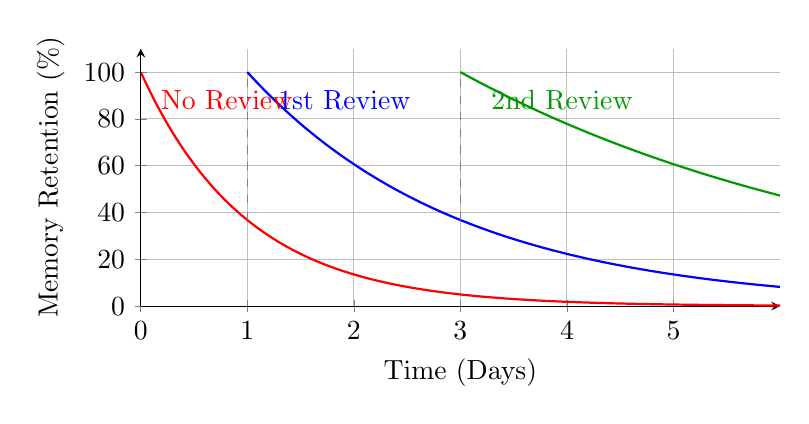
\begin{tikzpicture}
    \begin{axis}[
        width=0.8\textwidth,
        height=0.4\textwidth,
        xlabel={Time (Days)},
        ylabel={Memory Retention (\%)},
        xmin=0, xmax=6,
        ymin=0, ymax=110,
        xtick={0,1,2,3,4,5},
        ytick={0,20,40,60,80,100},
        axis lines=left,
        grid=major,
        smooth
    ]
    % Initial learning
    \addplot[color=red, thick, domain=0:6, samples=100] {100*exp(-x)};
    % First review
    \addplot[color=blue, thick, domain=1:6, samples=100] {100*exp(-0.5*(x-1))};
    \draw[dashed, gray] (1, 36.78) -- (1, 100);
    % Second review
    \addplot[color=green!60!black, thick, domain=3:6, samples=100] {100*exp(-0.25*(x-3))};
    \draw[dashed, gray] (3, 36.78) -- (3, 100);
    \node[anchor=south west, text=red] at (0.1, 80) {No Review};
    \node[anchor=south west, text=blue] at (1.2, 80) {1st Review};
    \node[anchor=south west, text=green!60!black] at (3.2, 80) {2nd Review};
    \end{axis}
\end{tikzpicture}
\caption{The Ebbinghaus Forgetting Curve illustrating the effect of spaced repetition on memory decay.}
\label{fig:ebbinghaus}
\end{figure}

\subsection{Automated Question Generation and Conversational AI}
Automated Question Generation (AQG) used to rely on syntax trees and manual templates, which often produced shallow questions \cite{kurdi2020systematic}. Transformer models changed this by understanding context better. For multiple-choice questions (MCQs), Kurdi et al. \cite{kurdi2020systematic} note that the difficulty lies in generating plausible distractors. A useful educational tool must generate distractors that are related to the topic but factually incorrect based on the text.

Integrating chatbot interfaces into educational tools provides a scalable way to support students \cite{winkler2020conversational}. Dan et al. \cite{dan2023educhat} demonstrated with the EduChat system that large-scale language models can successfully emulate Socratic tutoring interactions. As Fiorella and Mayer \cite{fiorella2015learning} note, explaining a concept is a generative activity that aids learning. Richard E. Mayer's Cognitive Theory of Multimedia Learning \cite{mayer2014cambridge} further suggests that combining visual and textual channels reduces cognitive overload, supporting the rationale for automated slide generation.

Table~\ref{tab:lit_summary} summarizes the key research concepts that guided the Lectura design.

\begin{table}[htbp]
\centering
\begin{tabular}{|l|p{5.5cm}|l|}
\hline
\textbf{Research Domain} & \textbf{Core Finding / Concept} & \textbf{Key Literature} \\ \hline
AI in Education & AI is best used as a cognitive support tool. & Luckin \cite{luckin2016intelligence}, Baidoo-Anu \cite{baidoo2023education} \\ \hline
Large Language Models & LLMs need strict contextual boundaries. & Kasneci \cite{kasneci2023chatgpt}, Wang \cite{wang2024large} \\ \hline
Context Grounding & RAG and CoT prompting reduce hallucinations. & Gao \cite{gao2023retrieval}, Wei \cite{wei2022chain} \\ \hline
Summarization & LLMs outperform older abstractive methods. & Liu \cite{liu2023summary}, See \cite{see2017get} \\ \hline
Cognitive Retrieval & Active recall and spaced repetition aid retention. & Roediger \cite{roediger2006test}, Cepeda \cite{cepeda2006distributed} \\ \hline
Question Generation & Plausible distractors are key for MCQ quality. & Kurdi \cite{kurdi2020systematic} \\ \hline
Conversational AI & AI tutors support generative learning behaviors. & Dan \cite{dan2023educhat}, Fiorella \cite{fiorella2015learning} \\ \hline
\end{tabular}
\vspace{6pt}
\caption{Summary of academic literature informing the Lectura framework.}
\label{tab:lit_summary}
\end{table}

\section{Review of Existing Solutions}
When developing a new educational platform, it is necessary to examine existing software solutions to understand current approaches and identify areas for improvement. The current market for study tools is fragmented into specialized applications. This section analyzes several major platforms across different categories, comparing their functionality to the proposed Lectura system.

\subsection{Methodology of Data Collection}
The competitive analysis was conducted using a mixed-methods empirical approach. Primary data was gathered through direct usability testing, where the author created active accounts on each target platform and attempted to process a standardized university lecture transcript. Secondary data was aggregated by reviewing official API documentation, published feature changelogs, and user-community forums to assess long-term platform stability and feature roadmaps. 

Executing a comprehensive competitor analysis presented notable challenges. First, several proprietary algorithms (such as the specific spaced-repetition multipliers used by Quizlet or the backend context-window parsing of Gamma.app) are closed-source, forcing the analysis to rely on black-box behavioral observation rather than code-level inspection. Second, rapid iteration cycles in generative AI mean that feature sets change weekly, creating a moving target for documentation.

\subsection{General-Purpose AI Assistants}
Notion AI integrates generative text features directly into the Notion workspace. It is primarily designed to help users write, summarize, and format notes within their existing databases. For students, Notion is useful for organizing information and generating quick summaries of text they have already typed.

However, Notion AI is optimized for general productivity rather than structured learning. It operates as a flexible text editor, but it does not have built-in algorithms for active recall or testing. From an engineering perspective, it lacks a dedicated ingestion pipeline for multimedia formats like video transcripts. Furthermore, it cannot natively generate academic formats like spaced-repetition flashcards or structured quizzes. While it is an excellent tool for storing notes, it does not actively participate in the student's memorization process.

ChatGPT has become a common tool for students to explain complex topics, summarize texts, and brainstorm ideas. The main limitation of using ChatGPT for regular studying is its lack of structure and persistence. To use it effectively, a student must manually copy and paste text (such as video transcripts), manage context limits, and write specific prompts to get the desired output format. This requires significant manual effort for every study session. In addition, ChatGPT does not save these outputs into an organized library of flashcards or quizzes. Lectura addresses this by automating the prompt engineering and file parsing processes, wrapping the LLM capabilities in a structured academic environment.

\subsection{Automated Slide Generators}
Gamma.app focuses on generating presentations and documents from text prompts. Unlike traditional software such as Microsoft PowerPoint, Gamma uses AI to automatically format content, create visual layouts, and organize text into readable slides. It is particularly effective at turning long paragraphs into structured visual presentations.

While Gamma is highly capable at creating visual slides, it functions in isolation from other study methods. A student cannot use Gamma to generate flashcards or practice tests from the same material. Lectura aims to incorporate this kind of automated slide generation alongside other tools. By doing so, a student can generate a presentation, a quiz, and a set of flashcards all from the same initial lecture transcript, without needing to export data to multiple different applications.

\subsection{Spaced Repetition and Flashcard Tools}
Quizlet is one of the most widely used platforms for digital flashcards and rote memorization. It provides features like the ``Learn'' and ``Test'' modes to help students memorize terms through repetitive practice. Recently, Quizlet added ``Q-Chat,'' an AI-assisted tool to help students study conversationally. Despite these features, Quizlet's main drawback is that it relies heavily on manual data entry. Students typically have to read a textbook or watch a lecture, manually identify key terms, and type them into the system one by one.

Anki is an open-source spaced repetition system (SRS) that uses scheduling algorithms to determine exactly when a student should review a flashcard to prevent forgetting. It is highly effective and widely used in demanding fields like medicine and language learning. However, Anki is known for having a steep learning curve and a complicated user interface. More importantly, like Quizlet, Anki requires the user to create their own cards or find community-made decks. It does not generate content. Lectura is designed to automate the card-creation step, allowing students to benefit from spaced repetition without spending hours manually creating the decks themselves.

\subsection{Online Learning Platforms}
Coursera provides access to video lectures, reading materials, and assignments from universities worldwide. It is a highly effective platform for delivering structured educational content to a large audience. The platform is designed primarily for content delivery rather than personalized revision. While students can watch lectures and take standard quizzes, Coursera does not automatically generate personalized study guides or flashcards based on the user's specific weaknesses. Lectura is designed to complement platforms like Coursera. A student can take the transcript from a Coursera lecture and input it into Lectura to generate localized, interactive study materials for that specific module.

\subsection{Comparative Synthesis and SWOT Analysis}
Each of the analyzed applications performs well in its specific area, but they often require students to use multiple disconnected tools. A student might use ChatGPT to summarize a lecture, Notion to store the notes, and Anki to memorize the terms. This fragmentation increases the administrative workload on the student.

To formalize the strategic positioning of Lectura within this competitive landscape, a SWOT (Strengths, Weaknesses, Opportunities, Threats) analysis was conducted, as visually summarized in Figure~\ref{fig:swot_matrix}.

\begin{figure}[htbp]
\centering
\begin{tikzpicture}[
    box/.style={draw=black, rectangle, minimum width=7cm, minimum height=3.5cm, align=left, text width=6cm, inner sep=10pt, fill=white},
    title/.style={anchor=north west, fill=black, text=white, font=\bfseries}
]
    % Strengths (Top Left)
    \node[box, thick] (S) at (0, 0) {
        \begin{itemize}[leftmargin=*, noitemsep]
            \item Automated, unified pipeline.
            \item Zero manual data entry.
            \item Bridges raw video to spaced repetition.
        \end{itemize}
    };
    \node[title] at (S.north west) {STRENGTHS};

    % Weaknesses (Top Right)
    \node[box, thick] (W) at (7.5, 0) {
        \begin{itemize}[leftmargin=*, noitemsep]
            \item Dependent on 3rd-party APIs.
            \item Lacks robust offline functionality.
            \item Strict context limits.
        \end{itemize}
    };
    \node[title] at (W.north west) {WEAKNESSES};

    % Opportunities (Bottom Left)
    \node[box, thick] (O) at (0, -4) {
        \begin{itemize}[leftmargin=*, noitemsep]
            \item LMS Integration.
            \item Live audio ingestion.
            \item Collaborative study groups.
        \end{itemize}
    };
    \node[title] at (O.north west) {OPPORTUNITIES};

    % Threats (Bottom Right)
    \node[box, thick] (T) at (7.5, -4) {
        \begin{itemize}[leftmargin=*, noitemsep]
            \item Tech giants natively integrating tools.
            \item Volatile AI API pricing.
        \end{itemize}
    };
    \node[title] at (T.north west) {THREATS};

\end{tikzpicture}
\caption{SWOT Analysis Matrix for the Lectura Platform.}
\label{fig:swot_matrix}
\end{figure}

Table~\ref{tab:feature_matrix} summarizes how Lectura compares to these existing platforms. By combining automated ingestion, visual slide generation, and algorithmic rehearsal into one system, Lectura attempts to streamline the study process, allowing students to focus on learning rather than managing software.

\begin{table}[htbp]
\centering
\resizebox{\textwidth}{!}{%
\begin{tabular}{|l|c|c|c|c|c|c|}
\hline
\textbf{Feature} & \textbf{Lectura} & \textbf{Gamma.app} & \textbf{Notion AI} & \textbf{Quizlet} & \textbf{Anki} & \textbf{ChatGPT} \\ \hline
Video Ingestion & Native API & Limited & None & Limited & None & Manual \\ \hline
Visual Slides & Auto/Gen & Yes & None & None & None & None \\ \hline
Summary Gen. & Templated & Document & Unstruct. & None & None & Manual \\ \hline
Auto Quizzes & Contextual & None & None & Yes, Basic & None & Manual \\ \hline
SRS Flashcards & Generated & None & None & User-Auth & User-Auth & None \\ \hline
Context. Chat & Anchored & None & Doc-level & Q-Chat & None & Stateless \\ \hline
\end{tabular}%
}
\vspace{6pt}
\caption{Feature comparison of Lectura against existing educational and productivity platforms.}
\label{tab:feature_matrix}
\end{table}

As the comparison shows, no single existing tool covers the full workflow from content ingestion to active recall testing. The following chapters describe the technical implementation of the Lectura platform.